
%\documentclass{vgtc}
\documentclass[journal]{vgtc}                % final (journal style)
%\documentclass[review]{vgtc}                 % review
%\documentclass[review,journal]{vgtc}         % review (journal style)
%\documentclass[widereview]{vgtc}             % wide-spaced review
%\documentclass[preprint]{vgtc}               % preprint
%\documentclass[preprint,journal]{vgtc}       % preprint (journal style)
%\documentclass[electronic]{vgtc}             % electronic version
%\documentclass[electronic,journal]{vgtc}     % electronic version, journal

%% Uncomment one of the lines above depending on where your paper is
%% in the conference process. ``review'' and ``widereview'' are for review
%% submission, ``preprint'' is for pre-publication, and the final version
%% doesn't use a specific qualifier. Further, ``electronic'' includes
%% hyperreferences for more convenient online viewing.

%% Please use one of the ``review'' options in combination with the
%% assigned online id (see below) ONLY if your paper uses a double blind
%% review process. Some conferences, like IEEE Vis and InfoVis, have NOT
%% in the past.

%% These three lines bring in essential packages: ``mathptmx'' for Type 1
%% typefaces, ``graphicx'' for inclusion of EPS figures. and ``times''
%% for proper handling of the times font family.
%% We encourage the use of mathptmx for consistent usage of times font
%% throughout the proceedings. However, if you encounter conflicts
%% with other math-related packages, you may want to disable it.

\usepackage{mathptmx}
\usepackage{graphicx}
\usepackage{times}
%\usepackage{tabularx}
\usepackage{amsmath}
%\usepackage{url}
\usepackage{subfigure}
\usepackage{multirow}
%\usepackage{teaser}

%% If you are submitting a paper to a conference for review with a double
%% blind reviewing process, please replace the value ``0'' below with your
%% OnlineID. Otherwise, you may safely leave it at ``0''.
\onlineid{0}

%% declare the category of your paper, only shown in review mode
\vgtccategory{Research}

%% allow for this line if you want the electronic option to work properly
\vgtcinsertpkg

%% In preprint mode you may define your own headline.
%\preprinttext{To appear in an IEEE VGTC sponsored conference.}

\usepackage{color}
\definecolor{RED}{rgb}{1,0,0}
\definecolor{BLUE}{rgb}{0,0,1}
\newcommand{\FIXME}[1]{\textbf{\color{BLUE}{FIXME: #1}}}
%\newcommand{\FIXME}[1]{}

% suppress  single floating lines on top (widow) and bottom (club)
%  10000 is infinity
%  tradeoff: possible underful vboxes
\clubpenalty=10000
\widowpenalty=10000

%% Paper title.
%----------------------------------------------------------------------
\title{Equalizer: A Mature Parallel Rendering Framework}
%----------------------------------------------------------------------

%% Author and Affiliation (multiple authors with multiple affiliations)
\author{Stefan Eilemann\thanks{email: eilemann@gmail.com} \\ %
\and Renato Pajarola\thanks{email: pajarola@acm.org}}

\affiliation{\scriptsize Visualization and MultiMedia Lab \\ Department of Informatics \\ University of Z\"urich}

%% Keywords that describe your work. Will show as 'Index Terms' in journal
%% please capitalize first letter and insert punctuation after last keyword
\keywords{Parallel Rendering, Scalable Visualization, Cluster Graphics, Immersive Environments, Display Walls}

%% ACM Computing Review (CR) categories.
%% See <http://www.acm.org/class/1998/> for details.
%% The ``\CRcat'' command takes four arguments.

\CRcatlist{ % not used in journal version
  \CRcat{I.3.2}{Graphics Systems}{Distributed Graphics}{Parallel Rendering};
  \CRcat{I.3.m}{Miscellaneous}{Rendering Clusters}{Scalable Rendering};
  \CRcat{I.3.7}{Three-Dimensional Graphics and Realism}{Virtual Reality}{Immersive Environments}
}

\vgtccategory{Research}

%% Copyright space is enabled by default as required by guidelines.
%% It is disabled by the 'review' option or via the following command:
% \nocopyrightspace

%%%%%% START OF THE PAPER %%%%%%
\begin{document}

%----------------------------------------------------------------------
%% Abstract section.
\abstract {
  We present the features, algorithms and system integration necessary to
  implement a parallel rendering framework usable in a wide range of real-world
  applications, based on the basic architecture and implementation of the Equalizer
  parallel rendering framework presented in \cite{EP:07}.
} % end of abstract

\maketitle

\begin{figure*}[ht]\center
  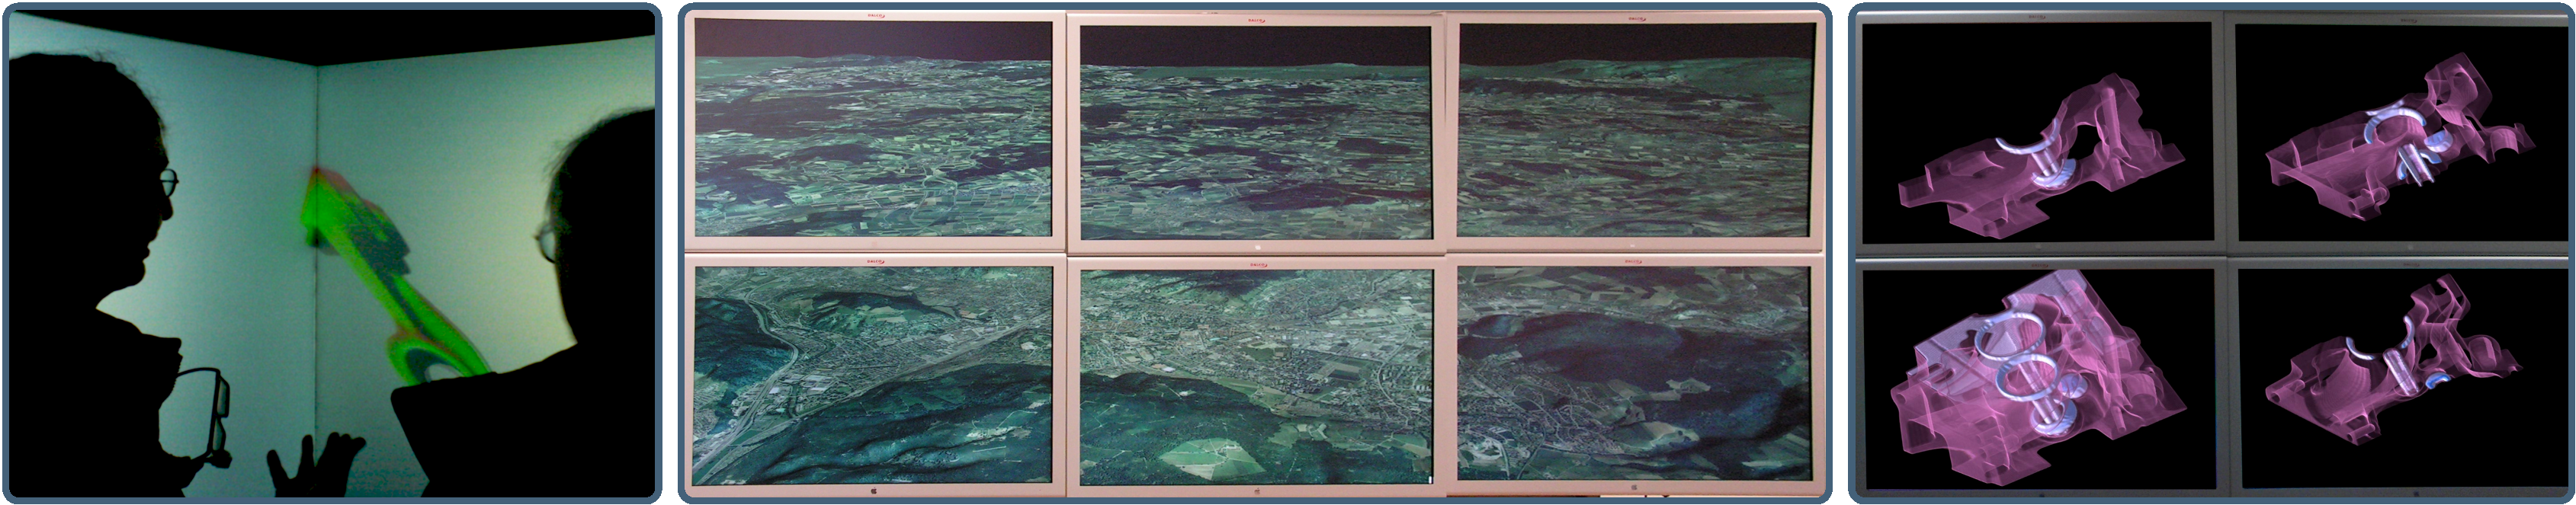
\includegraphics[width=2\columnwidth]{images/teaser} \\
  (a) \hfil \hfil (b) \hfil \hfil (c)
  \vspace{-2mm}
  \caption{Various Equalizer use cases: (a) immersive CAVE, (b) display wall and
    (c) scalable volume rendering.}
  \label{FIG_teaser}
\end{figure*}

%----------------------------------------------------------------------
\section{Introduction}
%----------------------------------------------------------------------

The continuing improvements in hardware integration lead to ever faster CPUs and GPUs, as well as higher resolution sensor and display devices. Moreover, increased hardware parallelism is applied in form of multi-core CPU workstations, massive parallel super computers, or cluster systems. Hand in hand goes the rapid growth in complexity of data sets from numerical simulations, high-resolution 3D scanning systems or bio-medical imaging, which causes interactive exploration and visualization of such large data sets to become a serious challenge. It is thus crucial for a visualization solution to take advantage of hardware accelerated scalable parallel rendering. In this systems paper we describe a new scalable parallel rendering framework called {\em Equalizer} that is aimed primarily at cluster-parallel rendering, but works as well in a shared-memory system. Cluster systems are the main focus  because workstation graphics hardware is developing faster than high-end graphics (super-) computers can absorb new developments, and also because clusters offer a better cost-performance balance.

Previous parallel rendering approaches typically failed in one of the following system requirements:
%
\begin{enumerate}\renewcommand{\labelenumi}{\alph{enumi})}
\addtolength{\itemsep}{-0.5\baselineskip}
\item generic application support, instead of special domain solution
\item scalable abstraction of the graphics layer
\item exploit existing code infrastructure, such as proprietary scene graphs, molecular data structures, level-of-detail and geometry databases
\end{enumerate}

To date, generic and scalable parallel rendering frameworks  that can be adopted to a wide range of scientific visualization domains are not yet readily available. Furthermore, flexible
configurability to arbitrary cluster and display-wall configurations has also not been addressed in the past, but is of immense practical importance to scientists depending high-performance interactive visualization as a scientific tool. In this paper we present Equalizer, which is a novel flexible framework for parallel rendering that supports scalable performance, configuration flexibility, is {\em minimally invasive} with respect to adapting existing visualization applications, and is applicable to virtually any scientific visualization application domain.

The main contributions that Equalizer introduces in a single parallel rendering system, and which are presented in this paper are:
%
\begin{enumerate}\renewcommand{\labelenumi}{\roman{enumi})}
\addtolength{\itemsep}{-0.5\baselineskip}
\item novel concept of compound trees for flexible configuration of graphics system resources,
\item easy specification of parallel task decomposition and image compositing choice through compound tree layouts,
\item automatic decomposition and distributed execution of rendering tasks according to compound tree,
\item support for parallel surface as well as transparent (volume) rendering through $z$-visibility as well as $\alpha$-blending compositing,
\item fully decentralized architecture providing network swap barrier (synchronization) and distributed objects functionality,
\item support for low-latency distributed frame synchronization and image compositing,
\item minimally invasive programming model.
\end{enumerate}

Equalizer is open source, available under the LGPL license from http://www.equalizergraphcis.com/, which allows it to be used both for open source and commercial applications. It is source-code portable, and has been tested on Linux, Microsoft Windows, and Mac OS X in 32 and 64 bit mode using both little endian and big endian processors.


%----------------------------------------------------------------------
\section{Related Work}
%----------------------------------------------------------------------
\label{SEC_related}

The early fundamental concepts of parallel rendering have been laid down in \cite{MCEF:94} and \cite{Crockett:97}. A number of domain specific parallel rendering algorithms and special-purpose hardware solutions have been proposed in the past, however, only few generic parallel rendering frameworks have been developed.

\subsubsection*{Domain specific solutions}

Cluster-based parallel rendering has been commercialized for off-line rendering (i.e. distributed ray-tracing) for computer generated animated movies or special effects, since the ray-tracing technique is inherently amenable to parallelization for off-line processing. Other special-purpose solutions exist for parallel rendering in specific application domains such as volume rendering \cite{LWMT:97,Wittenbrink:98,HSCSM:00,SL:02,GS:02,NSJLYZ:05} or geo-visualization \cite{VR:91,AG:95,LDC:96,JLMV:06}. However, such specific solutions are typically not applicable as a generic parallel rendering paradigm and do not translate to arbitrary scientific visualization and distributed graphics problems.

Recently in \cite{NC:07}, parallel rendering of hierarchical level-of-detail (LOD) data has been addressed and a solution specific to sort-first tile-based parallel rendering has been presented. While the presented approach is not a generic parallel rendering system, basic concepts presented in \cite{NC:07} such as load management and adaptive LOD data traversal can be carried over to other sort-first parallel rendering solutions.

\subsubsection*{Special-purpose architectures}

Traditionally,  high-performance real-time rendering systems have relied on an integrated proprietary system architecture, such as the SGI graphics super computers. These special-purpose solutions have become a niche product as their graphics performance does not keep up with off-the-shelf workstation graphics hardware and scalability of clusters. However, cluster systems need more sophisticated parallel graphics rendering libraries, such as the one proposed in this paper.

Due to its conceptual simplicity, a number of special-purpose image compositing hardware solutions for sort-last parallel rendering have been developed. The proposed hardware architectures include Sepia \cite {MHS:99a,sepia}, Sepia~2 \cite{LMSBHa:01,LMSBH:01}, Lightning~2 \cite{Stoll01}, Metabuffer \cite{Blanke00,Zhang01}, MPC Compositor \cite{Muraki01} and PixelFlow \cite{Molnar92, Eyles97}, of which only a few have reached the commercial product stage (i.e. Sepia~2 and MPC Compositor). However, the inherent inflexibility and setup overhead have limited their distribution and application support. Moreover, with the recent advances in the speed of CPU-GPU interfaces, such as PCI Express and other modern interconnects, combinations of software and GPU-based solutions offer more flexibility at comparable performance.

% FlowVR \cite{AGLLMRR:04}, not really related that much here

\subsubsection*{Generic approaches}

A number of algorithms and systems for parallel rendering have been developed in the past. On one hand, some general concepts applicable to cluster parallel rendering have been presented in \cite{Mueller:95,Mueller:97} (sort-first architecture), \cite{SZFLS:99,SFLS:00} (load balancing), \cite{SFL:01} (data replication), or \cite{CMF:05,CM:06} (scalability). On the other hand, specific algorithms have been developed for cluster based rendering and compositing such as \cite{AP:98}, \cite{CKS:02} and \cite{YYC:01,SMLAP:03}. However, these approaches do not constitute APIs and libraries that can readily be integrated into existing visualization applications, although the issue of the design of a parallel graphics interface has been addressed in \cite{Igehy98}.
%
Only few generic APIs and (cluster-) parallel rendering systems exist which include VR Juggler \cite{BJHMBC:01} (and its derivatives), Chromium \cite{HHNFAKK:02} (an evolution of \cite{Humphreys99,Humphreys00,HEBSEH:01}) and OpenGL Multipipe SDK \cite{JDBJBCER:04,BRE:05,MPK}.

VR Juggler \cite{BJHMBC:01,JBBC:98} is a graphics framework for virtual
reality applications which shields the application developer from the
underlying hardware architecture, devices and operating system. Its main
aim is to make virtual reality configurations easy to set up and use
without the need to know details about the devices and hardware
configuration, but not specifically to provide scalable parallel
rendering. Extensions of VR Juggler, such as for example ClusterJuggler
\cite{BC:03} and NetJuggler \cite{AGLMR:02}, are typically based on the
replication of application and data on each cluster node and basically
take care of synchronization issues, but fail to provide a flexible and
powerful configuration mechanism that efficiently supports scalable
rendering as also noted in \cite{SWNH:03}. The presented system is different from VR Juggler in that it
fully supports scalable parallel rendering such as sort-first and
sort-last task decomposition and image compositing, it provides more
flexible node configurations which for example allow specifying
arbitrary task decomposition and image compositing combinations as
simple compound layouts. Furthermore, it it is fully distributed which includes
support for network swap barriers (synchronization), distributed objects
as well as image compression and transmission. In contrast to VR
Juggler, Equalizer supports multiple rendering threads per process,
which is important for multi-GPU systems.

While Chromium \cite{HHNFAKK:02} provides a powerful and transparent
abstraction of the OpenGL API, that allows a flexible configuration of
display resources, its main limitation with respect to scalable
rendering is that it is focused on streaming OpenGL commands through a
network of nodes, often initiated from a single source. This has also been
observed in \cite{SWNH:03}. The problem
comes in when the OpenGL stream is large in size, due to not only
containing OpenGL calls but also the rendered data such as geometry
and image data. Only if the geometry and textures are mostly static
and can be kept in GPU memory on the graphics card, no significant
bottleneck can be expected as then the OpenGL stream is composed of a
relatively small number of rendering instructions. However, as it is
typical in real-world visualization applications, display and object
settings are interactively manipulated, data and parameters may change
dynamically, and large data sets do not fit statically in GPU memory but
are often dynamically loaded from out-of-core and/or multiresolution
data structures. This can lead to frequent updates not only of commands and
parameters wich have to be distributed but also of
the rendered data itself (geometry and texture), thus causing the OpenGL stream
to expand dramatically. Furthermore, this stream of function calls and
data must be packaged and broadcast in real-time over the network to
multiple nodes for each rendered frame. This makes CPU performance and
network bandwidth a more likely limiting factor. While preserving a minimally
invasive API, the novel proposed system is better aimed at scalability
as the actual data access is decentralized in the distributed rendering
clients.

The performance experiments in \cite{HHNFAKK:02} indicate that Chromium is working
quite well when the rendering problem is fill-rate limited.
This is due to the fact that the OpenGL commands and a non-critical
amount of rendering data can be distributed to multiple nodes without significant problems
and since the critical fill-rate work is then performed locally on the graphics hardware.

Chromium also provides some facilities for parallel application
development, namely a sort-last, binary-swap compositing SPU and an
OpenGL extension providing synchronization primitives, such as a barrier
and semaphore. It leaves other problems, such as configuration, task
decomposition as well as process and thread management unaddressed, thus
making the development of parallel OpenGL applications harder than with
Equalizer. Parallel Chromium applications tend to be written for one
specific parallel rendering use case, such as for example the sort-first distributed
memory volume renderer \cite{BHPB:03} or the sort-last parallel
volume renderer raptor \cite{Raptor}. We are not aware of a generic Chromium-based
application using many-to-one sort-first or stereo decompositions. This is
another difference to Equalizer which provides a much more flexible
task decomposition configuration. Applications written once for Equalizer can
easily be run in any different task decomposition mode and for any physical
display configuration without any changes to the application itself.
While Equalizer provides an abstraction of all entities of the rendering pipeline
(see Sections~\ref{SEC_architecture} and~\ref{SEC_development}), Chromium's
infrastructure is primarily the compositing stage.

OpenGL Multipipe SDK (MPK) \cite{BRE:05} implements an effective
parallel rendering API for a shared memory multi-CPU/GPU system. It is
similar to IRIS Performer \cite{RH:94} in that it handles multi-pipe
rendering by a lean abstraction layer via a conceptual callback
mechanism, and that it runs different application tasks in
parallel. However, MPK is not designed nor meant for rendering nodes
separated by a network. MPK focuses on providing a parallel rendering
framework for a single application, parts of which are run in parallel
on multiple rendering channels, such as the culling, rendering and final
image compositing processes. Compared to MPK, Equalizer supports a
fully distributed parallel rendering paradigm and features a more flexible
task decomposition approach.


%------------------------------------------------------------------------------
\section{Usability}
%------------------------------------------------------------------------------

\subsection{Physical and Logical Visualization Setup}

Canvas, Layout, Observer

multi-view with runtime switching,

2D overlays

Swap Barriers

\subsection{Auto-Configuration}

hwsd with VirtualGL support

\subsection{Sequel}

application, renderer, view data

\subsection{Qt Windowing}

Challenges in threading model, architecture

\subsection{Tide Integration}

Tiled interactive display environment, parallel pixel streaming, events

%------------------------------------------------------------------------------
\section{The Collage Network Library}
%------------------------------------------------------------------------------

\subsection{Distributed, Versioned Objects}

types (instance, delta, static), versioning, multicast, compression,
serializable with dirty bits, mapping, blocking commits

\subsection{Reliable Stream Protocol}

UDP-based reliability protocol

\subsection{Infiniband RDMA}

reverse-engr impl

%------------------------------------------------------------------------------
\section{Virtual Reality}
%------------------------------------------------------------------------------

\subsection{Dynamic Focus Distance}

Focus what user is looking at

\subsection{Asymmetric Eye Position}

Better HMD by measuring user geometry

\subsection{Application-specific Scaling}

Gullivers world

\subsection{Runtime Stereo Switch}

\subsection{Swap Synchronization and GPU affinity}

%------------------------------------------------------------------------------
\section{Performance}
%------------------------------------------------------------------------------

\subsection{New Decomposition Modes}

The initial version of Equalizer implemented sort-first (2D), sort-last (DB) and
stereo (EYE) decomposition. In the following we present new decomposition modes
and motivate their use case.

\subsubsection{Time-Multiplex}

Interaction with threading

\subsubsection{Tiles and Chunks}

Equalizers do what?

\subsubsection{Pixel}

Equal load for fill-limited apps

\subsubsection{Subpixel}

MSAA and DOF, plus idle refinement algo

\subsection{Equalizers}

Equalizer are one addition to compound trees. They modify parameters of their
respective subtree at runtime to optimize one aspect of the decomposition.

\subsubsection{Sort-First and Sort-Last Load Equalizer}

reactive load equalization, describe tunables (damping, resistance, delta,
granularity), sort-first respects input channel size

\subsubsection{Cross-Segment Load Equalizer}

summarize \cite{EEP:11}

\subsubsection{Dynamic Frame Resolution}

Constant frame rate for fill-limited applications

\subsubsection{Frame Rate Equalizer}

Predominantly used by DPlex to smooth output framerate

\subsubsection{Monitoring}

Control workstation in VR setups

\subsection{Optimizations}

\subsubsection{Region of Interest}

for compositing and load equalizer.

\subsubsection{Asynchronous Readback}

pipelines rendering with compositing

\subsubsection{Download and Compression Plugins}

GPU-CPU transfer plugins with optional compression (eg YUV) linked to CPU
compression for network transfer

\subsubsection{Thread Synchronization Modes}

Per-node sync, draw sync, async

%----------------------------------------------------------------------
\section{Applications}
%----------------------------------------------------------------------

\subsection{Livre}
\subsection{RTT Deltagen}
\subsection{RTNeuron}

%----------------------------------------------------------------------
\section{Experimental Results}
%----------------------------------------------------------------------
\label{SEC_results}

%----------------------------------------------------------------------
\section{Discussion and Conclusion}
%----------------------------------------------------------------------
\label{SEC_conclusions}


%----------------------------------------------------------------------
%\section*{Acknowledgements}
%----------------------------------------------------------------------
%% if specified like this the section will be ommitted in review mode
\acknowledgements{
We would like to thank and acknowledge the following institutions and projects for providing the 3D geometry and volume test data sets:
the Digital Michelangelo Project, Stanford 3D Scanning Repository, Cyberware Inc., volvis.org and the Visual Human Project.
This work was partially supported by the Swiss National Science Foundation Grant 200021-116329/1.
}

\vspace{-2mm}
\footnotesize
\bibliographystyle{abbrv}
\bibliography{references}

\end{document}
